\documentclass[a4paper,11pt]{article}
\usepackage[latin1]{inputenc}
\usepackage[T1]{fontenc}
\usepackage{bbm}
\usepackage{amsmath}
\usepackage{indentfirst}
\usepackage{fullpage}
\usepackage{url}
\usepackage{graphicx}
\usepackage[center,footnotesize]{caption}
\usepackage[section]{placeins}
\usepackage{subfig}
\title{Series 4 - solutions}
\date{}
\author{Genomics and bioinformatics - Week 5 - October 16, 2012}
\begin{document}
\maketitle

\section{Hidden Markov Model}
\begin{enumerate}
\item There are two states, say $I$ (isochore) and $N$ (normal). We observe sequences of bases A, T, G and C. For this exercise one can group G and C in one variable ``GC'', and similarly A and T in ``AT''. Note that from each state, the outgoing probabilities must sum to 1.

\begin{center}
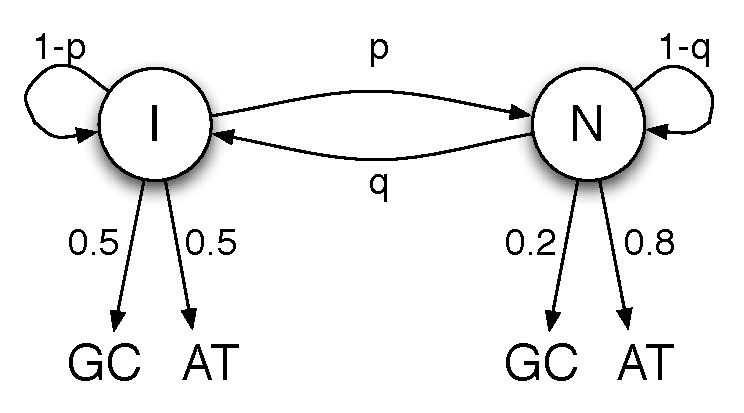
\includegraphics[height=0.2\textwidth]{hmm.pdf}
\end{center}

\item In state $I$ (isochore), the probability to see GC is 0.5, the same for AT. From state $N$, the probabilities are 0.2 for GC and 0.8 for AT.
\item The isochore is 7000 bases long, the genome 23'000'000, so the probability for a random base in the genome to belong to the isochore is $x = P(I) = 7'000/23'000'000 = 3\cdot 10^{-4}$.
\item We have
$$ P(N|I)=p; \ P(I|N)=q; \ P(I|I)=(1-p); \ P(N|N)=(1-q)$$
$$ P(I) = P(I|N)P(N) + P(I|I)P(I) $$
$$ P(N) = P(N|I)P(I) + P(N|N)P(N) $$
so in terms of $x$, $p$ and $q$:
$$ x = q(1-x) + (1-p)x $$
$$ 1-x = px + (1-q)(1-x) $$
Note that the two equations are equivalent, so one cannot solve directly for p and q.
\item From state $I$, one can consider the event ``staying in $I$'' as a fail, with probability $1-p$, and ``going to $N$'' as a success, with probability $p$. The number $X$ of failures before the first success is given by a geometric distribution:
$$ P(X=k) = (1-p)^k p .$$
Its mean is $E[X] = \frac{1-p}{p}$ (another formulation, taking $X$ as the time of the first success, leads to $E[X] = \frac{1}{p}$).
\footnote{\url{http://en.wikipedia.org/wiki/Geometric_distribution}}
\item If the isochore is generated from a geometric process as in the previous point, its length is most probably the mean of the distribution. So $7000 = E[X] = \frac{1-p}{p} \Rightarrow p = \frac{1}{7001}$ (or $\frac{1}{7000}$ with the alternative formulation), confirming what one could expect intuitively. Taking $p=\frac{1}{7000}$, one deduces from point 4 that $q = x/(1-x) p = \frac{1}{11496500}$. One may also compute $q$ as follows: Exchanging the role of $I$ and $N$ in point 5, writing $Y$ for the corresponding random variable and $L$ for the average length of the two non GC-rich regions, one obtains $L= \frac{23000000-7000}{2}$, $E(Y)=L_{\rm total}=2L$ and $E(Y) =  \frac{1-q}{q}$, so that $q = \frac{1}{11496500}$ as before.
\end{enumerate}

\section{Reading frame}

See the program "series5\_solution.py".

%%%%%%%%%%%%%
\section{BLAST}
%%%%%%%%%%%%%

(Results here may change with the evolution of sequencing databases).

\subsection{Nucleotide BLAST}

\begin{enumerate}
\item Do you get any matches to \texttt{fragment\_007}? Which parameters did you use? Record the alignment statistics for the top hits.

- Using the Nucleotide Collection (nr/nt) Database and optimizing for ``more dissimilar sequences''
(discontiguous megablast)

\vspace{0.5cm}
\begin{center}
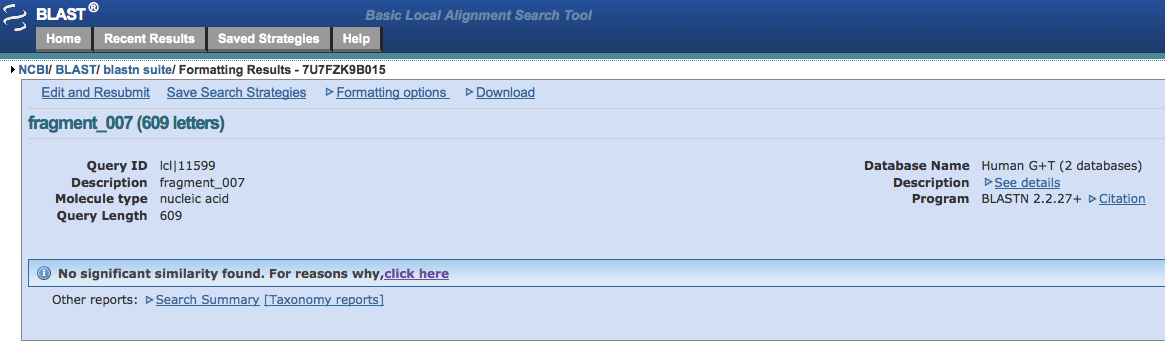
\includegraphics[width=0.8\textwidth]{blastn1.png}
\end{center}
\vspace{0.5cm}

\item Extract the sequence of the hit with the highest query coverage (this may not necessarily be the top hit) and perform another nucleotide BLAST, using the same parameters. Record the alignment statistics for the top hits.

\vspace{0.5cm}
\begin{center}
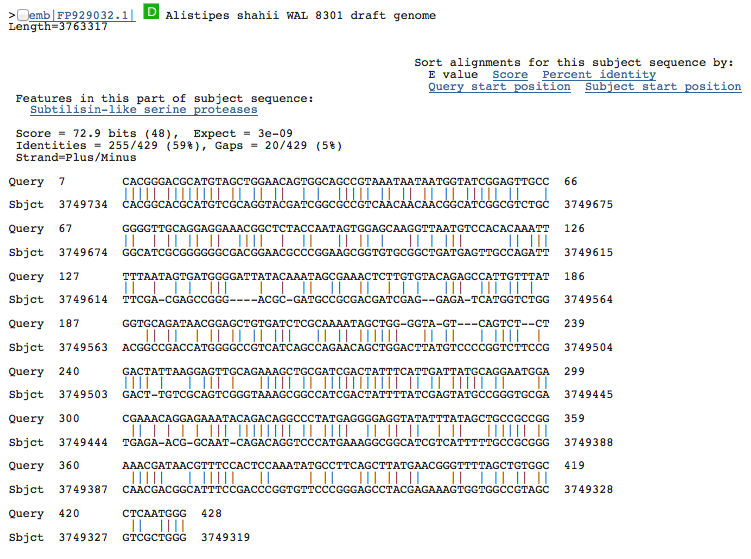
\includegraphics[width=0.8\textwidth]{blastn2.png}
\end{center}
\vspace{0.5cm}

\item What changes do you observe in the E-values? To which parameter could you attribute the these changes?  

- Improvement in the E-values. Parameter - Query coverage.

\item What is the default threshold for the E-value on NCBI BLAST?

- 10

\item Do you have any significant hits suggesting a possible function for \texttt{fragment\_007}? 

- The E-values are not significant. 

\end{enumerate}

\subsection{Protein BLAST}

\begin{enumerate}
\item Using your custom function from exercise 2, one can extract the following nucleotides sequence from the translation of the forward strand with shift 0 (must start with `M'; incomplete): \\ \texttt{MSTQIFNSDGDYTNSETLVYRAIVYGADNGAVISQNSWGSQSLTIKELQKAAIDYFIDYAGMDETGEIQT \\ GPMRGGIFIAAAGNDNVSTPNMPSAYERVLAVASMGPDFTKASYSTFGTWTDITAPGGDIDKFDLSEYGV \\ LSTYADNYYAYGEGTSMACPHVAGAA}.\\
Copy it into a file \texttt{aa\_007.fasta}, or directly into the BLASTp interface, and run the alignment. After a few seconds, you get the following matches of the peptidases S8 S53 superfamily:

\vspace{0.5cm}
\begin{center}
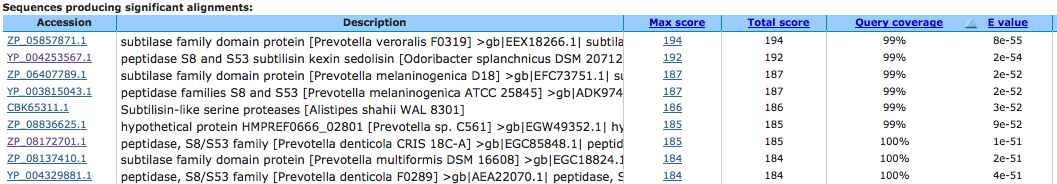
\includegraphics[width=0.8\textwidth]{blastp.png}
\end{center}
\vspace{0.5cm}

\item \texttt{fragment\_007} encodes for a subtilase family domain protein. It is a member of the peptidases S8 (subtilisin and kexin) and S53 (sedolisin) family. These include endopeptidases and exopeptidases.

\item  \emph{Odoribacter, Prevotella, Porphyromonas} and \emph{Alistipes} species are predominant. Note that \emph{Alistipes} is the one you found with the nucleotide BLAST, and it is not the top match.

\item BLASTx

\item Amino acid sequences are more conserved than nucleotide sequences. Often even the highest-scoring subject sequences retrieved using the nucleotide sequence will cover only small regions of the query sequence, while quite often the corresponding sequences retrieved using the amino acid sequence will cover more of the gene.

\end{enumerate}

\subsection{Finding orthologs}

Specify in the \textit{Organism} section of the BLASTp interface that you want to align on species \emph{Candida glabrata}. Consistently with the publication, the best match indicates \\ 
\texttt{GENE ID: 2890989 CAGL0L07436g}:

\vspace{0.5cm}
\begin{center}
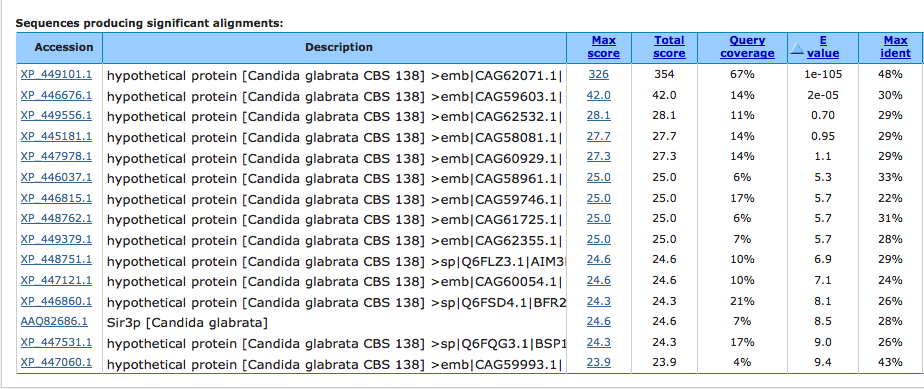
\includegraphics[width=0.8\textwidth]{blastp_ortholog.png}
\end{center}
\vspace{0.5cm}

\end{document}
